\documentclass{beamer}
\mode<presentation>
\usepackage{amsmath}
\usepackage{amssymb}
%\usepackage{advdate}
\usepackage{graphicx}
\graphicspath{{../figs/}}
\usepackage{adjustbox}
\usepackage{subcaption}
\usepackage{enumitem}
\usepackage{multicol}
\usepackage{mathtools}
\usepackage{listings}
\usepackage{url}
\def\UrlBreaks{\do\/\do-}
\usetheme{Boadilla}
\usecolortheme{lily}
\setbeamertemplate{footline}
{
  \leavevmode%
  \hbox{%
  \begin{beamercolorbox}[wd=\paperwidth,ht=2.25ex,dp=1ex,right]{author in head/foot}%
    \insertframenumber{} / \inserttotalframenumber\hspace*{2ex} 
  \end{beamercolorbox}}%
  \vskip0pt%
}
\setbeamertemplate{navigation symbols}{}
\let\solution\relax
\usepackage{gvv}
\lstset{
%language=C,
frame=single, 
breaklines=true,
columns=fullflexible
}

\numberwithin{equation}{section}



\begin{document}

\title{9.4.33}
\author{EE25BTECH11020 - Darsh Pankaj Gajare}
% \maketitle
% \newpage
% \bigskip
%\begin{document}
{\let\newpage\relax\maketitle}
%\renewcommand{\thefigure}{\theenumi}
%\renewcommand{\thetable}{\theenumi}

Question:\\ Find the roots of the following quadratic equation graphically.
$x^2-4x+3$\\
\solution

The parabola can be expressed in matrix form as
\begin{align}
	\vec{x}^\top \vec{V} \vec{x} + \vec{u}^\top\vec{x} + f = 0
\end{align}
where
\begin{align}
	\vec{V} = \myvec{1 & 0 \\ 0 & 0}, \quad 
    \vec{u} = \myvec{-4 \\ -1}, \quad 
    f = 3.
\end{align}
The line $y=0$ is expressed as:
\begin{align}
    \vec{x} = \vec{q} + \lambda \vec{m}, \quad 
    \vec{q} = \myvec{0 \\ 0}, \quad 
    \vec{m} = \myvec{1 \\ 0}.
\end{align}

Substituting
\begin{align}
	(\vec{q} + \lambda\vec{m})^\top \vec{V} (\vec{q} + \lambda\vec{m}) 
    + \vec{u}^\top(\vec{q} + \lambda\vec{m}) + f = 0.
\end{align}
\begin{align}
	\lambda^2 \brak{\vec{m}^\top \vec{V} \vec{m}}
	+ \lambda \brak{2\vec{q}^\top \vec{V} \vec{m} + \vec{u}^\top \vec{m}}
	+ \brak{\vec{q}^\top \vec{V} \vec{q} + \vec{u}^\top \vec{q} + f} = 0.
\end{align}
\begin{align}
	\vec{m}^\top \vec{V} \vec{m} &= 1, \\
	2\vec{q}^\top \vec{V} \vec{m} + \vec{u}^\top \vec{m} &= -4, \\
	\vec{q}^\top \vec{V} \vec{q} + \vec{u}^\top \vec{q} + f &= 3.
\end{align}

\begin{align}
    \lambda^2 - 4\lambda + 3 = 0.
\end{align}

\begin{align}
    \lambda_1 = 1, \quad \lambda_2 = 3.
\end{align}

Thus, the intersection points are
\begin{align}
    \vec{x}_1 = \myvec{1 \\ 0}, \quad 
    \vec{x}_2 = \myvec{3 \\ 0}.
\end{align}
\begin{frame}
Plot using C libraries:
\begin{figure}[H]
	\centering
	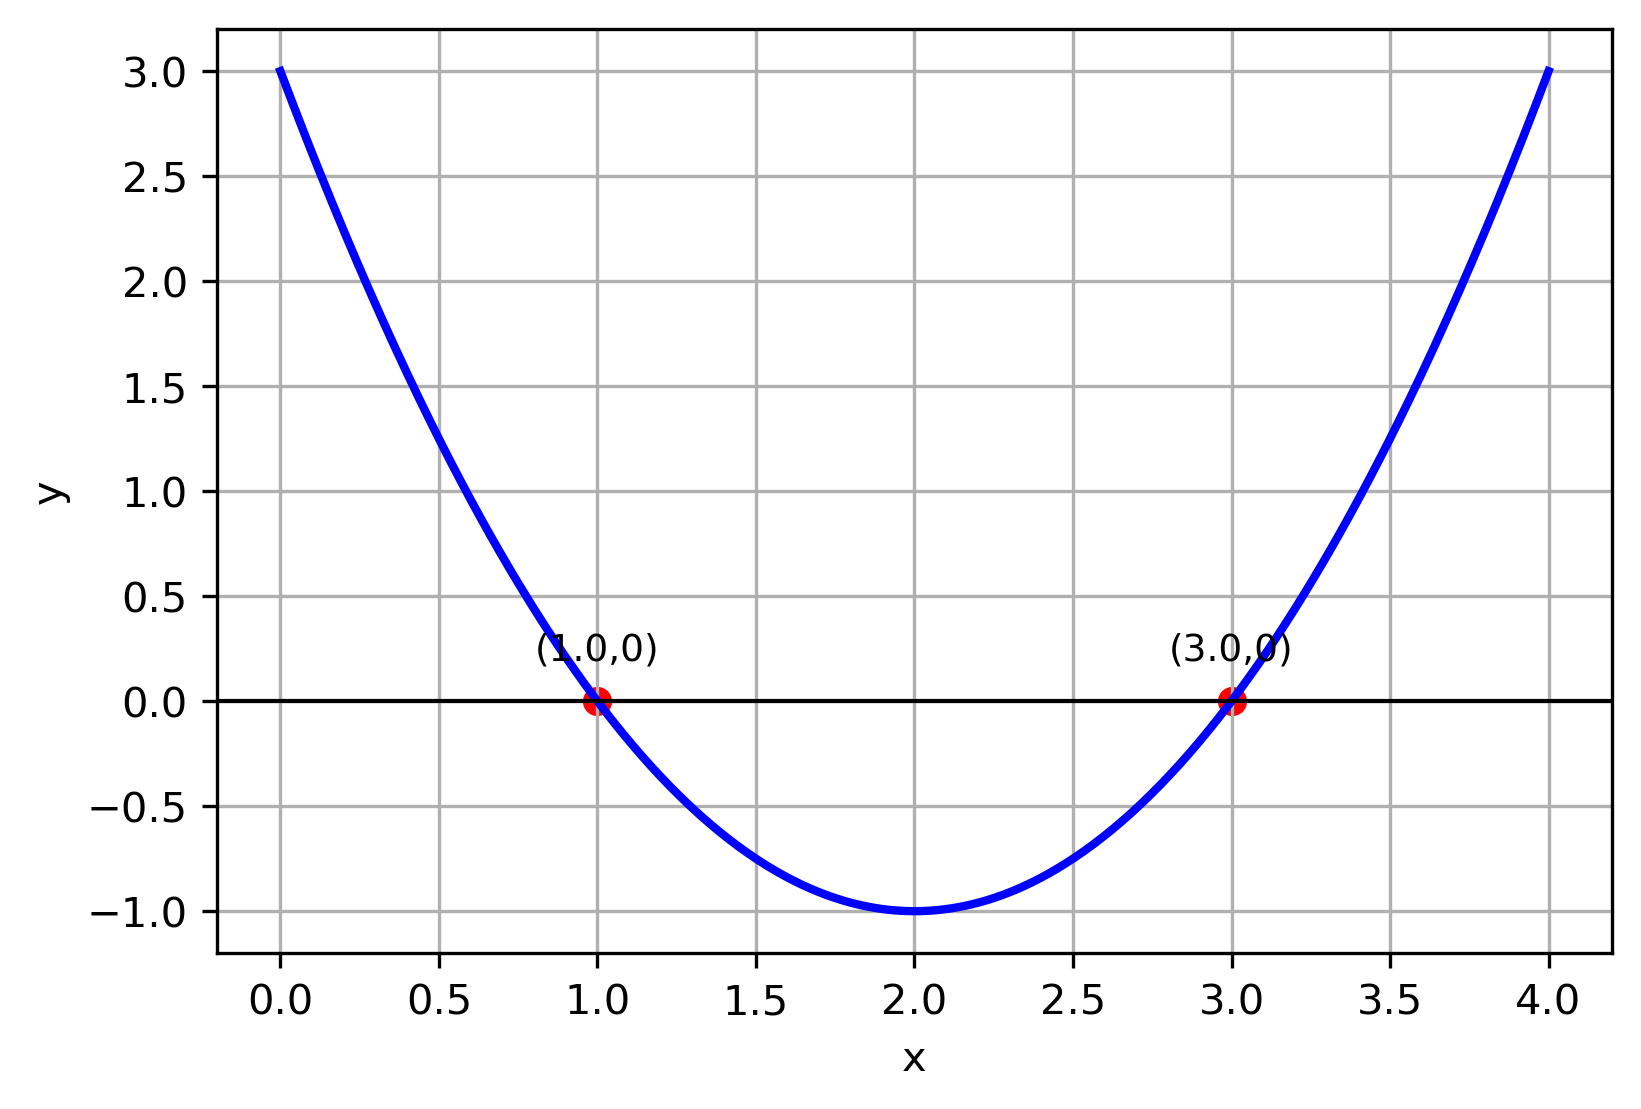
\includegraphics[scale=0.5]{img1}
	\caption*{}
	\label{img1}
\end{figure}
\end{frame}
\begin{frame}
Plot using Python:
\begin{figure}[H]
	\centering
	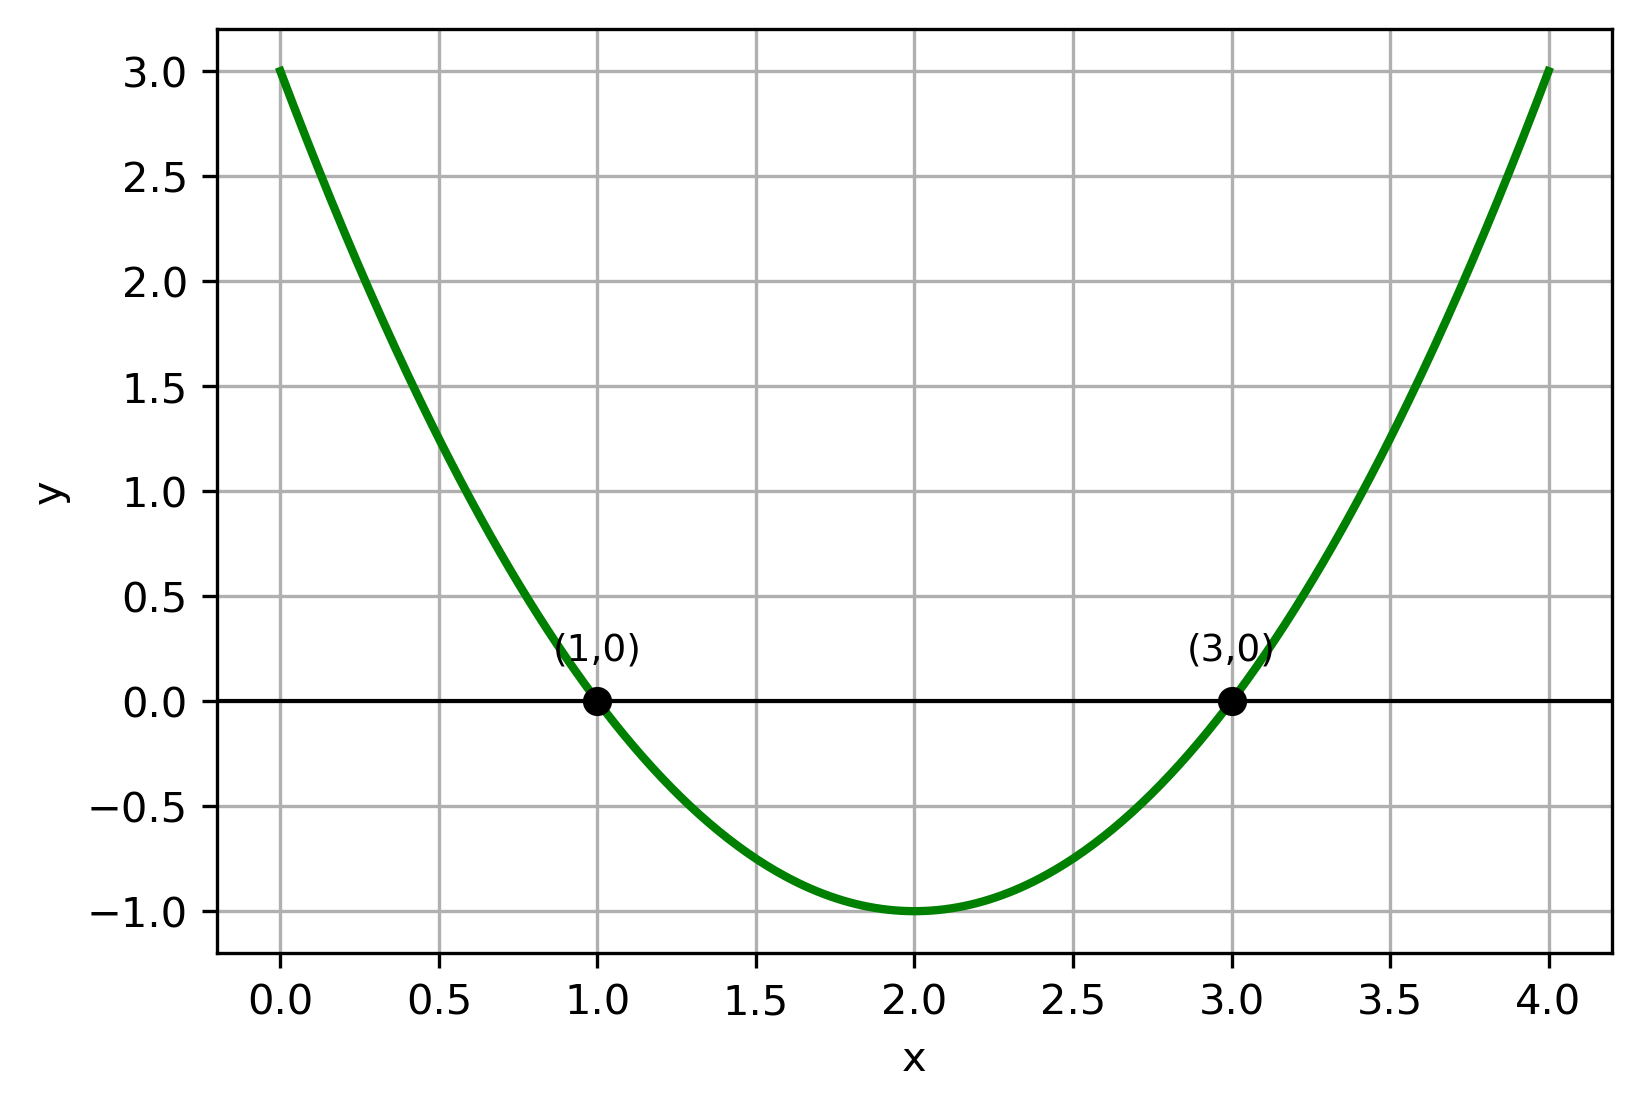
\includegraphics[scale=0.5]{img2}
	\caption*{}
	\label{img2}
\end{figure}
\end{frame}
\end{document}

